
\section{Series 1}
\subsection{Exercise 1}
\subsubsection{Question a}
The set $\mathcal{F}$ is built according the following rules, $\forall
A \subseteq \Omega$, with $\Omega$ a countably infinite set:
\begin{enumerate}
\item $|A| < \infty \rightarrow A \in \mathcal{F}$
\item $A \in \mathcal{F} \rightarrow A^c \in \mathcal{F}$
\end{enumerate}
\begin{proof}
  We try to make some attempt to study the minimal composition of
  $\mathcal{F}$, induced by its definition.

  By rule 1, $\emptyset \in \mathcal{F}$ holds because $|\emptyset| <
  \infty$. By rule 2 follow $\Omega \in \mathcal{F}$, because
  $\emptyset \in \mathcal{F}$ and $\Omega = \emptyset^c$. So far we
  have $\mathcal{F} = \{\emptyset, \Omega \}$. Using rule 1 again,
  every finite set $A \subset \Omega$ belong to $\mathcal{F}$, hence
  $\mathcal{F} = \{\emptyset, \Omega \} \cup \{A \subset \Omega:
  |A|<\infty\}$. But the sets we added in the last step in
  $\mathcal{F}$ allow us to apply rule 2 on each of them, forcing to
  add the complement of each: $\mathcal{F} = \{\emptyset, \Omega \}
  \cup \{A \subset \Omega: |A|<\infty\} \cup \{A^c \subset \Omega:
  |A|<\infty\}$ (note that the set $A^c$ is infinite where $A$ is
  finite and $\Omega$ is coutably infinite).

  The definition of $\mathcal{F}$ doesn't allow to add any other sets,
  hence we stop here in its construction.

  To show that $\mathcal{F}$ is not trivial, we have to show that
  exists a set which is in $2^{\Omega}$ but not in $\mathcal{F}$. In
  order to find such set, we have to exclude any finite set because by
  definition and the argument described above, it belong to
  $\mathcal{F}$. Hence it must be an infinite set. But we cannot
  choose an infinite set which is the complement of a finite one,
  otherwise it is in $\mathcal{F}$ too. Hence the choice restrict to
  an infinite set $A$ such that both $A$ both $A^c$ (which is infinite
  too, otherwise $A \in \mathcal{F}$ by rule 1) are not in
  $\mathcal{F}$. The set that contains every pair of sets $A$ and
  $A^c$, both infinite, is $2^\Omega$ and this finish the proof.
\end{proof}
To make an example choose $\Omega = \mathbb{N}, A = \{2i:i \in
\mathbb{N}\}$.

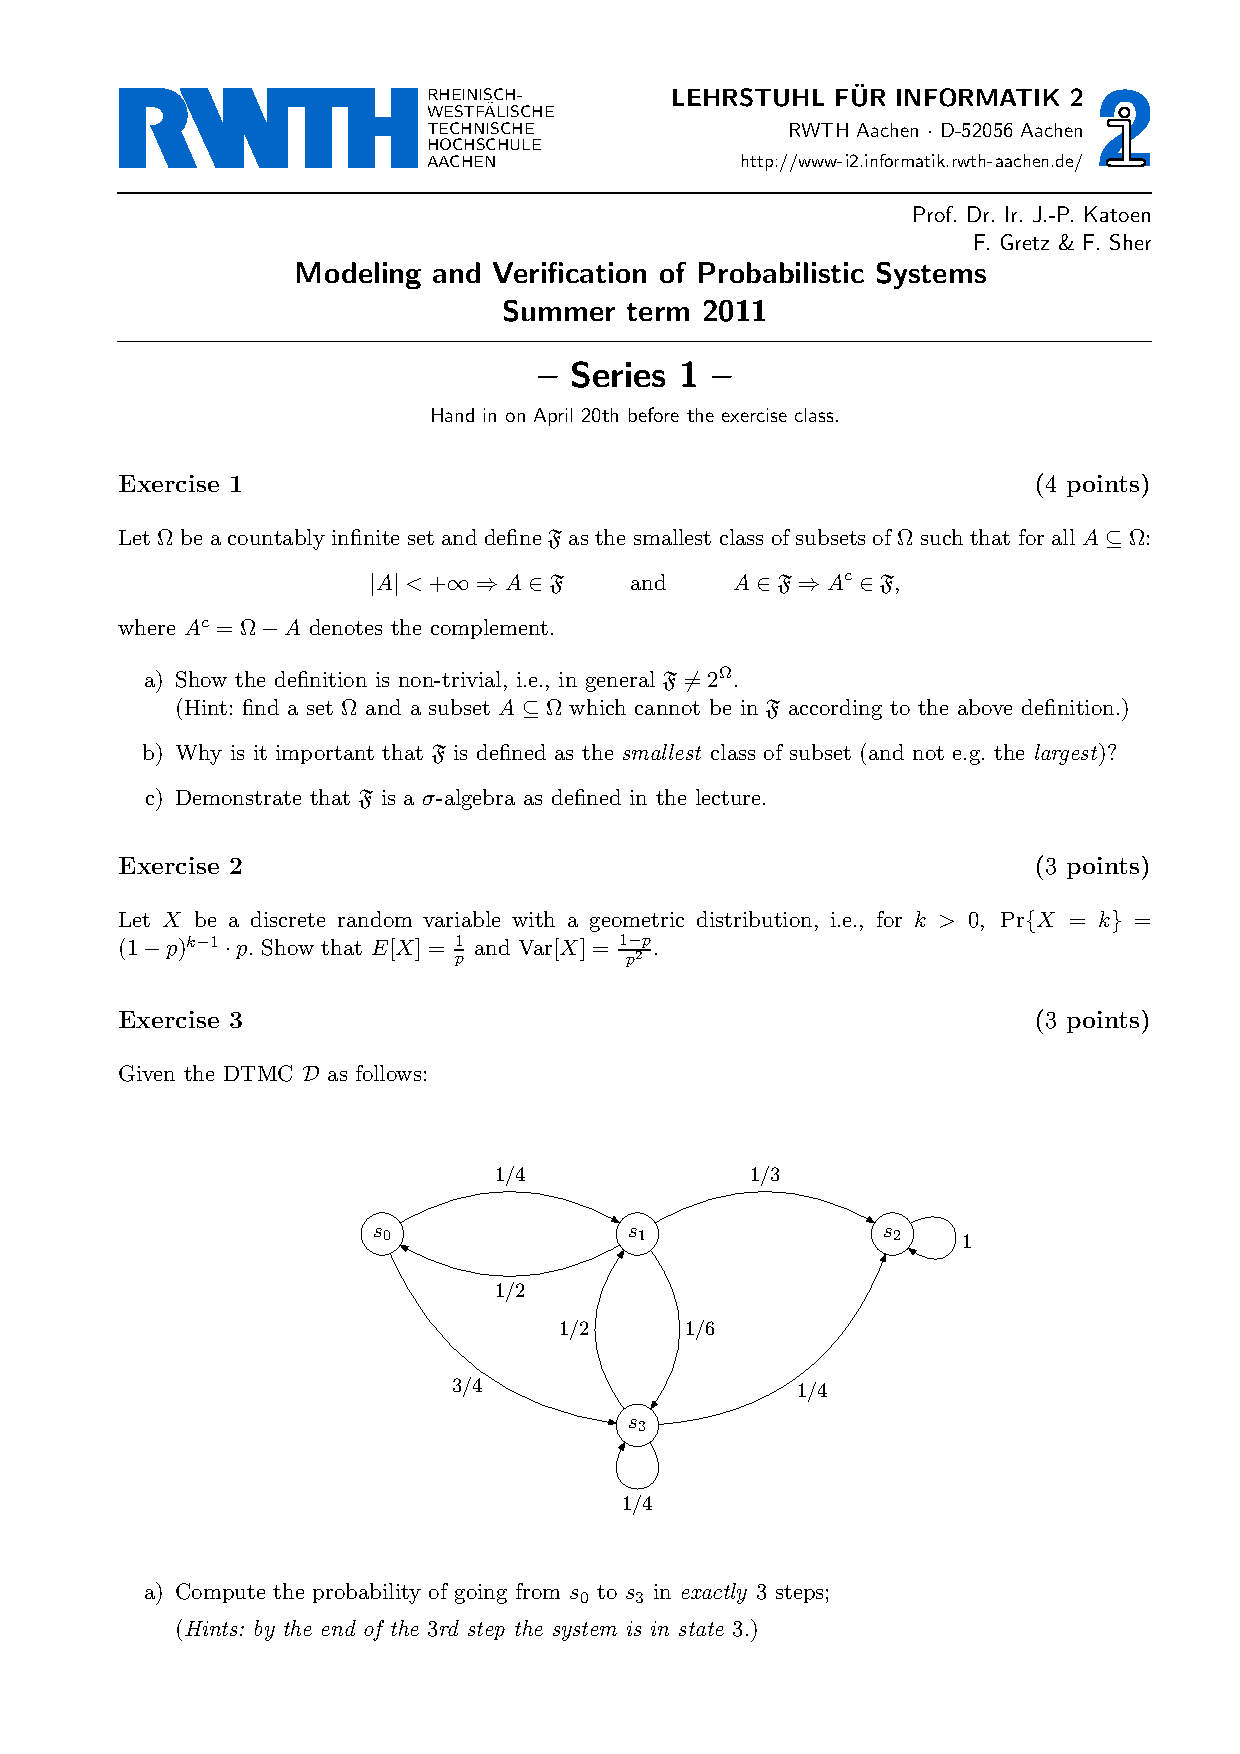
\includepdf[pages={-}]{pdf-to-include/sheet01.pdf}

\subsubsection{Question b}
It is important that $\mathcal{F}$ is defined as the \emph{smallest}
class of subset because the constraint ``smallest'' allow our building
process to stop where we mention before, that is, it allow to not
include pairs of sets $A$ and $A^c$ both infinite. This is the main
difference between $\mathcal{F}$ and $2^\Omega$, having a non trivial
set $\mathcal{F}$.

It is important to note that given $\Omega$ a countably infinite set,
$\mathcal{F}$ is countably infinite too, because the number of finite
sets (which all belong to $\mathcal{F}$) is infinite.

Instead, if the ``largest'' constraint was required, we have to
include as many sets as we can, every pairs of sets $A$ and $A^c$,
both infinite, too. In this way we have $\mathcal{F} = 2^\Omega$, so
the definition of $\mathcal{F}$ would be trivial.

\subsubsection{Question c}
Recall the definition of $\sigma$-algebra: a pair $(\Omega,
\mathcal{F})$, with $\Omega \not = \emptyset$ and $\mathcal{F}
\subseteq 2^\Omega$, is a $\sigma$-algebra if:
\begin{enumerate}
\item $\Omega \in \mathcal{F}$
\item $A \in \mathcal{F} \rightarrow A^c \in \mathcal{F}$
\item $\left( \forall i\in\{1,\ldots, n\}: A_i \in \mathcal{F} \right)
  \rightarrow \left(\bigcup_{i=1}^{n} A_i \right ) \in \mathcal{F}$
\end{enumerate}
In the following we show that $\mathcal{F}$ is a $\sigma$-algebra.
\begin{proof}
  By our argument of \emph{Question a}, $\Omega \in \mathcal{F}$ holds
  and by rule 2 of $\mathcal{F}$'s definition, $A \in \mathcal{F}
  \rightarrow A^c \in \mathcal{F}$ holds too. For the last point we
  reason case by case, given $A_i, A_j$ sets both in $\mathcal{F}$:
  \begin{itemize}
  \item if $A_i$ and $A_j$ are both finite, the union of finite sets
    is also finite, hence by rule 1 of $\mathcal{F}$'s definition,
    $A_i \cup A_j \in \mathcal{F}$ holds;
  \item if $A_i$ is finite and $A_j$ is infinite, their union is
    infinite (that is, $A_i \cup A_j$ is the complement of some finite
    set $A_k$). But given an infinite set $A$, we saw before that $A
    \in \mathcal{F} \leftrightarrow |A^c| < \infty$ holds. Using rule
    1, $|A^c| < \infty \rightarrow A^c \in \mathcal{F}$ and so $A_i
    \cup A_j \in \mathcal{F}$ too;
  \item if $A_i$ and $A_j$ are infinite (they're the complements of
    some finite sets $A_i^c, A_j^c$ respectively), their union is
    infinite, so we apply the argument given in the previous point.
  \end{itemize}
\end{proof}

\subsection{Exercise 3}
\subsubsection{Question a}
We type it directly in R:
\begin{lstlisting}
> P <- rbind(c(0, 1/4, 0, 3/4),
+            c(1/2, 0, 1/3, 1/6),
+            c(0, 0, 1, 0),
+            c(0, 1/2, 1/4, 1/4))
> temp <- c(1, 0, 0, 0) # initial distribution all on the zero state
> temp <- temp %*% P # compute the probability distribution after one step
> temp <- temp %*% P # compute the probability distribution after two steps
> temp <- temp %*% P # compute the probability distribution after three steps
> temp # see the result
       [,1]      [,2]     [,3]      [,4]
[1,] 0.1875 0.1458333 0.453125 0.2135417
\end{lstlisting}
The probability to be in $s_3$ starting from $s_0$ in \emph{exactly}
three step is about $.21$.

\subsubsection{Question c}
We type it directly in R:
\begin{lstlisting}
> P <- rbind(c(0, 1/4, 0, 3/4),
+            c(1/2, 0, 1/3, 1/6),
+            c(0, 0, 1, 0),
+            c(0, 1/2, 1/4, 1/4))
> temp <- c(.25, .25, .25, .25) # initial uniform distribution
> temp <- temp %*% P # compute the probability distribution after one step
> temp <- temp %*% P # compute the probability distribution after two steps
> temp <- temp %*% P # compute the probability distribution after three steps
> temp # see the result
           [,1]      [,2]      [,3]      [,4]
[1,] 0.08854167 0.1223958 0.6397569 0.1493056
\end{lstlisting}
The probability to be in $s_2$ in \emph{exactly} three step, assuming
a starting uniform distribution, is about $.63$.
